\section{Self loops}
%///////////////////////////////////////////////////////////
%*** Self loops ***
%	- the reduction tend to suppress self loops in transient transitions:
%		. ie in order to have self loops, you need to have U(n) = U(n-1)
%		. suppress all the transients that last not so long
%		. in another scenario, the only way to suppress self loops in transiant states is to increase the state discretization
%		%% example of the second integrator that needs 2 steps to go backward
%		%% plot the case of the reduced model that have overlapps
%		%% show the second int model discretization that we need for it.
%
%		. overlapps:
%			¤ show a graph of what is happening in the velocity between the dbl and dbl1r
%			¤ say that it force us to increase the number of cells in the second case to see what is happening
%///////////////////////////////////////////////////////////
%
Let a trajectory $\{p_i,\u_i\}_{i\in \mathbb{N}}$ of the abstraction $\sysa$.
If at timestep $n$ the trajectory is taking a self loop transition in the abstraction:
\begin{equation}
(\tuple{P,\pastuseq})
\systransition{\sysa}{\u_n}
(\tuple{P,\pastuseqn})
\end{equation}
then the input sequence verify $(\tuple{\pastuseqn}) = (\tuple{\pastuseq})$.
This means that self loops only appear when the control input is constant over time.

For an unobserved dynamic of the system that is damped in less than $\Ninputs$ timesteps, the abstraction will never create any self loops corresponding to the transient state.
% How to go from this result on the abstraction to the suppression of self loops?
% I need to make a link between the abstraction non reduced (the fact that we will have to consider self loops and that the reduction can just consider them in an efficient way)

\section{Size of the abstraction}
%///////////////////////////////////////////////////////////
%*** Size of the state space / FTS ***
%	In 2 parts: study of the number of nodes, then of the number of edges
%
%	- memories are really bad (not so sure) for the state space representation (they you need to consider all the past events) 
%		. compare the size of the state space for the original model and the previous one
%		. fixed points number depends on the state size
%		-> just underline the fact that the size of a set of nodes in a rectangle have also the set of all the inputs and as the algorithm is based on it
%		then the complexity is growing fastly
%		. give a formula on the number of nodes, it will be much better for understanding it
%		. compare it to any models
%
%	- study when it worth it to add memories or when it will just increase the size of the state space
%		. explain when it worth to use reachable sets from invariants or from observation -> link it to the model
%		%% make 2 curves about it: one will be the reachable set from the invariant, the other will be from the observation
%		. show that the one with the invariant is always more over approximated than the one with the observation
%		. there is a link between this and the noise (basically we can model more noise because there is some more space between the lyapunov function and the other estimation)
%///////////////////////////////////////////////////////////
%

\subsection{State space size}
The size of the state space of the reduced abstraction is mainly dependant on the cardinality of the set $\U$ (or the cardinality of its discretization).
The size of the state space is equal to $\Nobs \card{\U}^{\Ninputs}$.
As the size of the state space is exponentially dependant on the number of memories for the input set, we should reduced it as much as possible (with the constraint of finding a feasible solution for the control synthesis problem).

\subsection{Size of the reached sets}
The complexity of graph algorithms is dependant on the number of edges.
In the case of the reduced abstraction, the number of successors is directly dependant on the size of the reachable sets $\Xunobs$.
Therefore, we will investigate how the volume of the set  $\Xunobs(\Pastuseq)$ is influenced by the number of input memory considered and by the sampling rate.

\renewcommand{\dt}{dT}
Lets define the variable $T = \Ninputs\dt$, where $\dt$ is the sampling time of the reduced abstraction.

In order to see the influence of the sampling rate, we will work on the continuous model. 
As the observed part of the system does not influence the unobserved part, we will adopt a general formulation for the asymptotically stable monotone linear system (how ever, such a study can be done as well in the case of non monotone systems thanks to lyapunov functions).
Let the following model:
\begin{equation}
\dot{\x} = A \x + B \u + E \w
\end{equation}
% Do I do the study with lyapunov functions of with monotones systems?
% Lyap:
% easy, can be done in an annexe
% got already a curve dependant on the sampling time and on the number of inputs

In the monotone case, the volume of successors is directly dependant on the bounds of the set $\Xunobs(\Pastuseq)$.
By computing:
\newcommand{\xs}{\msup{\xunobs}}
\renewcommand{\xi}{\minf{\xunobs}}
\newcommand{\Dx}{\Delta \x}
\newcommand{\Du}{\Delta \u}
\newcommand{\Dw}{\Delta \w}
\begin{equation}
\begin{split}
\xs(T) &= \traj{T,\xs,\u(t),\msup{\w}} \\
\xi(T) &= \traj{T,\xi,\u(t),\minf{\w}} \\
\end{split}
\end{equation}
Thanks to the linearity of the differential equations, we have:
\begin{equation}
\msup{\xunobs}(T) - \minf{\xunobs}(T)
= \traj{T,
\msup{\xunobs}- \minf{\xunobs}
,\uo,
\msup{\w} - \minf{\w}
}
\end{equation}
we can then express the quantity $\Dx(T) = \msup{\xunobs}(T) - \minf{\xunobs}(T)$ with:
\begin{equation}\label{eq:vect_succ}
\begin{split}
\Dx(T) &= \Dx(0) \exp{A T} + \int_{0}^{T} \exp{A t} dt E \Dw \\
\Dx(0) &= A^{-1}(B \Du + E \Dw) \\
\end{split}
\end{equation}
The volume $V$ of the set $[\xi(T),\xs(T)]$ does not depend on the input sequence. As the set $[\xi(T),\xs(T)]$  is a rectangle, $V$ is equal to the product of all the component of the vector $\xs(T) - \xi(T)$.
\begin{equation}
V = \prod_{i=1}^{n} \Dx_i
\end{equation}
The volume of successor is evolving at the same speed than the dynamics.

If we observe the state $\xunobs$, then the only difference that it will make on equation \ref{eq:vect_succ} is that $\Dx(0) = \vect{0}$.
This mean that the number of successors is always smaller for the observed abstraction than for the reduced abstraction.

Figure \ref{fig:successor_volume} show the volume of successors evolve.
As the decay time of the speed controller is equal to $0.5s$, after this time, the volume of successors is almost the same for the 2 models.
So it is better to use the reduced model. If the sampling time $\dt \approx 0.5s$ then by choosing $\Ninputs\geq1$ we will create an abstraction that is small and that take in account the transient time. For $\dt\gg0.5s$, not observing the controlled variable seems to be possible as the number of successors between the 2 models are almost the same. If $\dt \ll 0.5s$, a good strategy would be to keep observing this variable.

\begin{figure}[!ht]
 %Experiment made on the quadruple tank process with values taken in the article of Johanson with 		T1,T2,T3,T4 = (63.,91.,5.,56.)
  \centering
  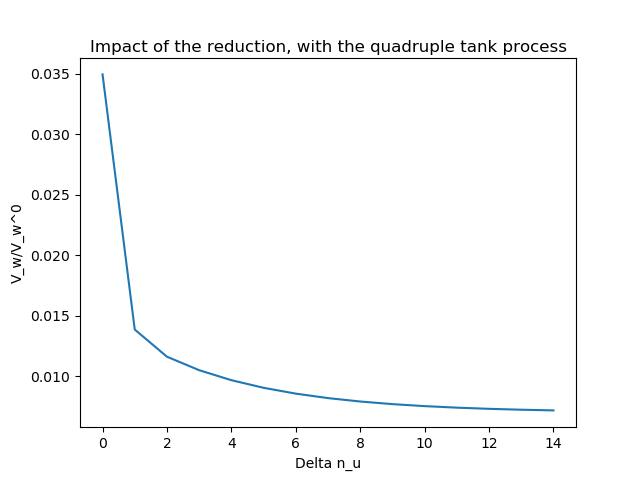
\includegraphics[width=0.9\linewidth]{lin_sys_reduction_seq_control_len}
  \caption{Impact of the variable $\Ninputs$ over the size of the possible state of the reduced system. It does not worth to take $\Ninputs$ greater than 1 since the boundaries of the reduce system does not decrease that much and the complexity of the model exponentially dependant of the number of controls.}
  \label{reduced_system_bounds}
\end{figure}
